\chapter{Documentation of the executable script \textsl{enkode}}
\thispagestyle{empty}
\label{enk}
{\texttt{2014} -- \texttt{2021}}

\bigskip
\smallskip
\setcounter{page}{17}

\noindent
\begin{info}
\begin{minipage}{0.95\textwidth}
\vspace{0.25cm}
This application as a command line falls within a developmental process as an \myulineyellow{\textsl{alpha version}} within an experimental research. Any feedback is therefore welcomed.
\vspace{0.25cm}
\end{minipage}
\end{info}

\section{Presentation}

\textsl{enkode} is an executable script Bash and it can be used as a command line under Unix or Linux. This executable consists to analysis a signal defined by a sound file according to some modalities that will be described here. 

This script was designed more specifically for undetermined pitch percussion music. Then, the modalities concern the analytic discrimination in terms of duration (sample segmentation), relative pitches (defined by $f0$ and the centroid) and dynamics (as loudness and low-pass filtered event loudness as `loudbass') in such a way each segment is analyzed as an array event. Thus, \textsl{enkode} generates data on the \textsl{stdout} for structural or formal analysis and sound synthesis as parameters.

This is an experimental procedure destinated to illustrate one way to extract relevant characteristics of a sonic segment.

\textsl{enkode} needs two main programs. The first one is Praat devoted to the analysis sound files, and the second one is the lisp compiler SBCL for data processing. The Shell script \textsl{enkode} insures the mediation.

\section{Event segmentation}
\label{enk:es}

\subsection{Dynamic profile}

Beforehand, we use the analysis of Praat software that has the particularity to process each analysis with a simple script. This script generates initially cochleagram analysis based on the perception of sound by the ear. This allows considering the same encoding of the inner ear to the brain. This translates into a bark scale\footnote{The Bark scale is a psycho-acoustical scale proposed by Eberhard Zwicker in 1961.} ranged in 24 critical bands of hearing, and the perceived sound level expressed in phone. The phonie is a weighted expression of the sound level according to an equal loudness curve (see figure \ref{fig:psycho}) which reflect the sensitivity of the human auditory system. The equal loudness curves have been empirically established in 1933 by Fletcher and Munson, and revised in 1956 by Robinson and Dadson.

\begin{figure}[!hbt]
	\begin{center}
		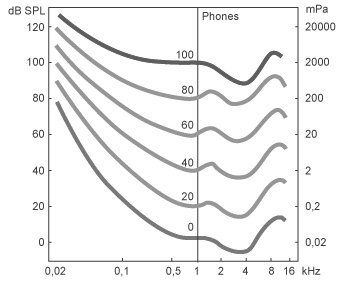
\includegraphics[scale=0.6]{img/5629}
		\caption{Equal loudness curves.}
		\label{fig:psycho}
	\end{center}
\end{figure}

To complete this representation of our sound perception, the phones of analysis Praat are converted into sones\footnote{The sone unit can estimate a sound twice as loud by a double value of loudness.} such as: 

\begin{equation}
sones= 2^{\frac{phones-40}{10}} \nonumber
\end{equation}

Thus, by adding the loudness of each frame (designating the timbre profile) we get a relevant dynamic profile.

\begin{figure}[!hbt]
	\begin{center}
		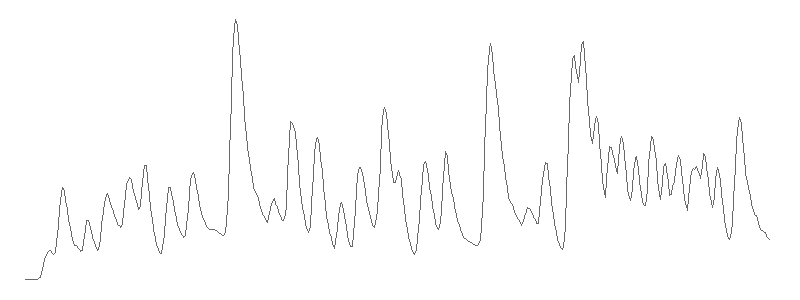
\includegraphics[width=\textwidth]{img/9832}
		\caption{Dynamic profile of a sample computed by Praat. [ $\rightarrow$ \ref{an:pro} ]}
		\label{fig:g1}
	\end{center}
\end{figure}

\subsection{TextGrid}

The TextGrid is a connected sequence of labeled intervals, with boundaries in between. Currently, these intervals correspond to an event.

From figure \ref{fig:g1}, we have to make a segmentation to discriminate each event inside the sample in order to write an appropriate TextGrid file that we will use for further analysis in Praat. For that we have to select each peak and each valley from the profile and fill the following conditions in the case where:
\begin{itemize}
\item If the sample start or finish on a peak -- for example, due to an inappropriate `cutting' -- it will be ignored.
\item The differential gap under a threshold loudness between consecutive peak and valley or valley and peak imply their removal. This gap can be set with \texttt{--loudness-diff-threshold} -- the default value is the mean value \myuline{according to the logarithmic scale} of the variations peak/valley and valley/peak.
\item All peak's level lower than a minimal loudness is deleted. This minimal value of loudness as peak can be set with \texttt{--loudness-min-threshold}. The default value is the minimum value of a peak after the filtering of \texttt{--loudness-diff-threshold}.
\item All valley's level upper than a maximal loudness is deleted. This maximal value of loudness as valley can be set with \texttt{--loudness-max-threshold}. The default value is the maximum value of a valley after the filtering of \texttt{--loudness-min-threshold}.
\item All event whose duration is less than the value of \texttt{--min-duration} -- 0.05 second by default -- will be merged with the next event, except for the last which will be merge in this atypical case with the previous event.
\item All event whose duration is more than the value of \texttt{--max-duration} -- 10 seconds by default -- will be truncated to fit within this duration.
\end{itemize}

\section{Extracting the required values}

Now, with the sample and its associate TextGrid, a script Praat allows getting values for each event as duration, $f0$, centroid, loudness and `loudbass'.

\subsection{Duration}

The duration of each event is estimated from the $\Delta t$ between two valleys of the profile as described above. The duration of the last peak is estimated from the last valley in relation to the total duration of the sample.

\subsection{\textit{f}0}

From each segment, we deduct the timbre profile by smoothing spectrum by the cepstrum method\footnote{\textbf{Smoothing spectrum by the cepstrum method}.\\ The signal can be viewed as a superposition of a short wave vibration with the `period' of $F0$ and long wave vibrations representing the course of the transmission function.\\
Then, smoothing means low-pass filtering the signal in such a way that the present short-wave vibration with the `period' of $F0$ is removed and the envelope remains. If $F0$ is known, a band-stop filter can be used instead of the low-pass, i.e., a filter that blocks only the undesired oscillations and their immediate vicinity, but lets everything else pass.}.

%\noindent
%\begin{info}
%\begin{minipage}{0.95\textwidth}
%\vspace{0.25cm}
%\textbf{Smoothing spectrum by the cepstrum method}\\
%The signal can be viewed as a superposition of a short wave vibration with the `period' of $F0$ and long wave vibrations representing the course of the transmission function.\\
%Then, smoothing means low-pass filtering the signal in such a way that the present short-wave vibration with the `period' of $F0$ is removed and the envelope remains. If $F0$ is known, a band-stop filter can be used instead of the low-pass, i.e., a filter that blocks only the undesired oscillations and their immediate vicinity, but lets everything else pass.
%\vspace{0.01cm}
%\end{minipage}
%\end{info}

\smallskip

The value of $F0$ in Praat is estimated to 500 Hz and can be set with the option \texttt{--smooth-frequency}.

\smallskip

Then, only the first peak or partial from the smoothed profile is retained as $f0$.

\subsection{Centroid}

The relative pitch is estimated -- currently in the case of an inharmonic sound -- by the centroid of the timbre profile as spectrum\footnote{The spectrum is a representation of a sound as either power or pressure as a function of frequency.} for a given sound event expressed in Hertz.

\smallskip

The spectral centroid represents the frequency center of gravity of a signal. The center of gravity is the average of $f$ over the entire frequency domain, weighted by the power spectrum. 

\smallskip

The centroid is defined as follow:

\begin{equation}
f_c=\frac{\displaystyle \int_0^\infty f P(f) df}{\displaystyle  \int_0^\infty P(f) df} \nonumber
\end{equation}

with $P(f)$ as the power spectrum.

\subsection{Loudness}

The loudness of a sound event is expressed in sone unit. 

\smallskip

Knowing that the loudness is defined for each frame such as:

\begin{equation}
L = \int 2^{(e(f)-40)} df \nonumber
\end{equation}

with $e(f)$ as the excitation in phon unit.

\smallskip

I state that for a continuous sound, the `amplitude' feeling decreases over time by habituation. The decreasing function is depending of the context and of the duration of the sound object. The first is not quantifiable and the second is moreover depending of the shape of the sound object. Therefore, intuitively and empirically as an experimental evaluation, the mean loudness of a given sound object is estimated as follow:

\begin{equation}
\overline{L}=\frac{\displaystyle \sum_{i=1}^{n}(n-i+1)L_{(i-1)dt}}{\displaystyle \sum_{i=1}^{n}i} \nonumber
\end{equation}

\subsection{Bass loudness}

In order to isolate the salience of bass frequencies as presence, we have to realize a filtering type low pass filter (figure \ref{fig:lpf}) and then get the loudness in the same way as seen previously with the loudness.

\begin{figure}[!hbt]
	\begin{center}
		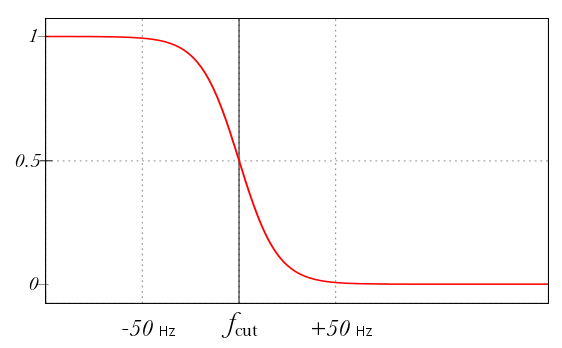
\includegraphics[scale=0.4]{img/4309}
		\caption{Low Pass Filter showing the width (fixed to +/- 50 Hz) of the region between pass and stop according to the cut off frequency.}
		\label{fig:lpf}
	\end{center}
\end{figure}

The cut off frequency can be set with the option \texttt{--cutoff-frequency} (default value is 100 Hz).

\section{Discrimination in classes}
\label{enk:dic}

The values generated by the previous analysis are destinated to be discriminated into $n$ classes in order to get a numerical score, mainly for structural analysis and as synthesis parameters.
This is done by a recursive discrimination based on the mean of the overall values.

\bigskip

Then, with the option \texttt{-I}, \texttt{--as-int}, the result is a data list of positive integers with by line an event, and by column respectively the class number of duration, $f0$, centroid, loudness and `loudbass'. Also, the result can be converted as a thrifty code\footnote{The thrifty code consists to write one information on one bit of n digits. This involves a discrimination of the order of $card(A_n) = n$.} with the option \texttt{-T}, \texttt{--as-tc}, or as a gray code\footnote{Gray code -- according to the Bell Labs researcher Frank Gray who introduced the term of \textit{reflected binary code} in 1947 -- is an ordering of the binary numeral system such that two successive values differ in only one bit.} with the option \texttt{-G}, \texttt{--as-gc}.

\bigskip

All these options take as argument a positive number which is applied as a number of recursivity for all different parameters, or a list of positive numbers as the number of recursivity with a cardinal equal to 5, that is to say one number by values of events.
Each class as positive integer means the value of an attractor. This ordered alist is written on the 5 first lines of \textsl{$<$fileName$>$.info}.

\bigskip

\begin{figure}[!hbt]
	\begin{center}
		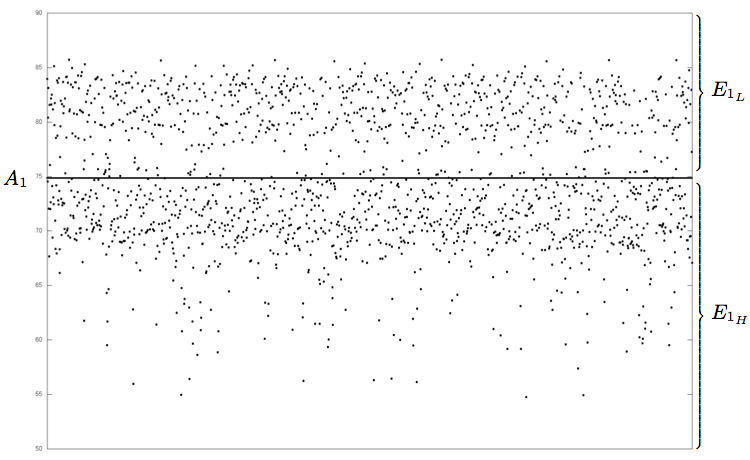
\includegraphics[scale=0.4]{img/1265}
		\caption{[Coefficient of recursivity: 1] In this example is represented by a cluster of bass loudness. The attractor $A_1$ is the arithmetic mean of all points, creating in this way two subsets: $E_{1_L}$ and $E_{1_H}$.}
		\label{fig:gb1}
	\end{center}
\end{figure}

\begin{figure}[!hbt]
	\begin{center}
		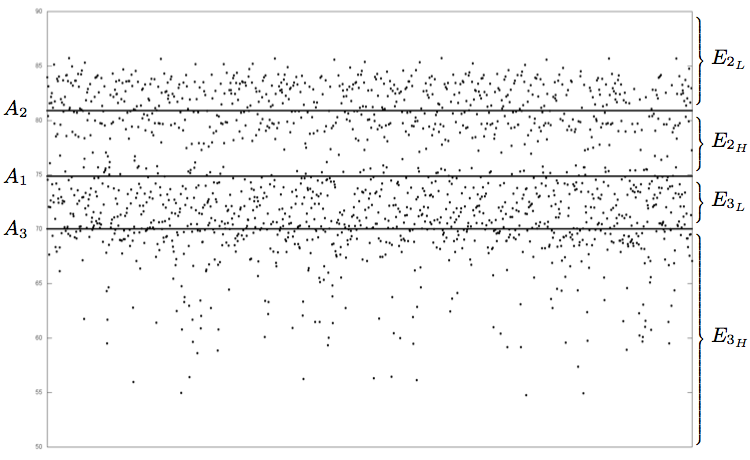
\includegraphics[scale=0.4]{img/1266}
		\caption{[Coefficient of recursivity: 2] From the two subsets of figure \ref{fig:gb1} ($E_{1_L}$ and $E_{1_H}$), we determine in the same manner two new attractors (respectively $A_2$ and $A_3$) generating in this way two subsets for each attractor, respectively $E_{2_L}$, $E_{2_H}$, $E_{3_L}$, and $E_{3_H}$.}
		\label{fig:gb2}
	\end{center}
\end{figure}

\begin{figure}[!hbt]
	\begin{center}
		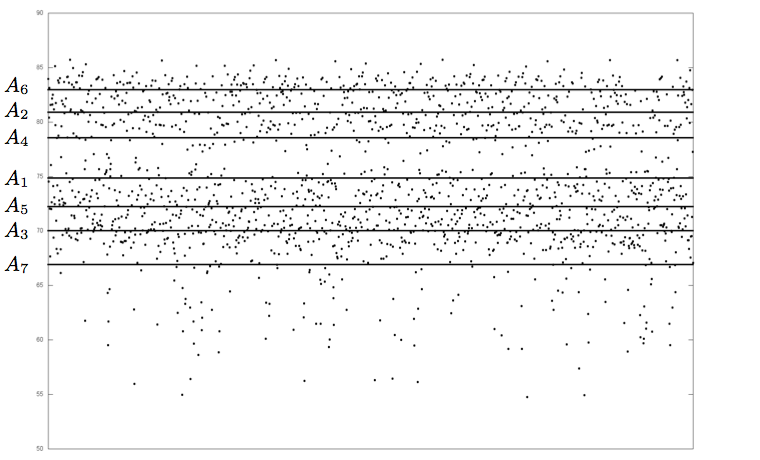
\includegraphics[scale=0.4]{img/1267}
		\caption{[Coefficient of recursivity: 3] Just repeat the process described above (see Figures \ref{fig:gb1} and \ref{fig:gb2}) to obtain 4 new attractors ($A_4$, $A_5$, $A_6$ and $A_7$) calculated from subsets of Figure \ref{fig:gb2}. This gives us a total of 7 attractors (or classes).}
		\label{fig:gb3}
	\end{center}
\end{figure}

\begin{figure}[!hbt]
	\begin{center}
		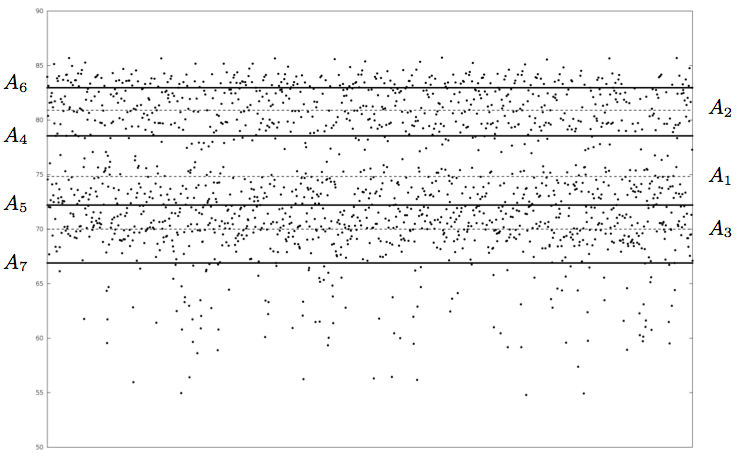
\includegraphics[scale=0.4]{img/1268}
		\caption{When the argument is a float number -- for example with a value of 2.5 -- the number of attractors is equal to a number of attractors with a coefficient of recursivity of 3 (ceiling value of 2.5) -- see figure \ref{fig:gb3} -- minus the number of attractors with a coefficient of recursivity of 2 (floor value of 2.5) -- see figure \ref{fig:gb3}. Thus, this gives us the 4 following attractors: $A_4$, $A_5$, $A_6$, and $A_7$.}
		\label{fig:gb4}
	\end{center}
\end{figure}

This way to discriminate data consists to determinate a number of classes relative to attractors. These attractors are computed by the arithmetic mean of the data in terms of the set according to a coefficient of recursivity determining the number of attractors. When the argument $n$ is an integer, the number of attractors is equal to $2^n - 1$ and when the argument $n$ is a float number, the number of attractors is equal to $2^{\lfloor n \rfloor}$.

\bigskip

See the description of this algorithm on figures \ref{fig:gb1} to \ref{fig:gb4}.

\noindent
\begin{info}
\begin{minipage}{0.95\textwidth}
\vspace{0.25cm}
Note that the recursivity stops when all data are captured by an attractor. Then, the number of discrimination can be smaller than the number of expected attractors defined by the value of the argument.%\\ 
%Also, mind that the number of discrimination is exponential, then you have to choose carefully this or these number(s).
\vspace{0.25cm}
\end{minipage}
\end{info}

\section{Command line use}

\subsection{Install \textsl{enkode}}

\begin{itemize}
\item Create a personal bin directory -- for instance \texttt{\$HOME/bin}
\item Copy \textsl{enkode} in this folder.
\item Add the following to file \texttt{$\sim$/.profile}\\ 
\texttt{export PATH=\$HOME/bin:\$PATH}

\item To install man page:
\begin{lstlisting}[language=bash]
$ sudo mkdir /usr/local/share/man/man1
$ sudo cp enkode.1 /usr/local/share/man/man1/
# plus on LINUX
$ sudo mandb
\end{lstlisting}
\end{itemize}
%$ sudo gzip /usr/local/share/man/man1/enkode.1

\subsection{Using \textsl{enkode}}

\begin{itemize}
\item Preliminary analysis
\begin{lstlisting}[language=bash]
$ enkode -p test.wav 
NumberOfEvents            119
--loudness-min-thres      14.955614       < 18.768398
--loudness-max-thres      46.377018       > 39.519974
--loudness-diff-thres     3.8155203       < 3.8345852 > 3.7744398
MinDiffLoudness           0.018797874
MaxDiffLoudness           48.29043
\end{lstlisting}
This table allows to adjust the different threshold values according to their initial value and their next efficient value.
Most of the time, these values have to be adjusted empirically according to the accuracy required.

\smallskip

Sometimes, the discriminative algorithm is not accurate or efficient enough. In this case, the segmentation can be edited or created in Praat. 
Then, it is recommended to `reframe' the TextGrid, that is to say labelled the first tier as an ordered integer. This can be done with the script \texttt{enkode.praat} -- see section \fullref{enkps}.
%In order to format the TextGrid as an ordered integer as label, it is recommended to apply the script \nameref{ftg} -- see appendice \fullref{ftg}.

\item Default behavior:
\begin{lstlisting}[language=bash]
$ enkode test.wav 
0.28 228.790283203125 235.7666500379242 8.830720512009613 1.7966619273740976  
0.10999999999999999 193.798828125 165.9317394706834 5.758170441172713 1.9914783596510206  
0.15999999999999998 506.0302734375 492.1692215465892 10.396071452511483 1.6476902981421457  
0.12 349.91455078125 374.6610256304264 10.416102008324566 1.6657044245205024  
0.14999996000000004 204.5654296875 206.9951008846426 9.59662211074838 1.9097877289745604     
...
\end{lstlisting}
\item Using some options:
\begin{lstlisting}[language=bash]
$ enkode --as-gc=3 test.wav
1 0 1 0 0 1 0 0 1 0 0 1 1 1 1  
0 0 1 0 0 1 0 0 1 0 0 1 1 0 0  
0 1 0 1 0 0 1 1 1 0 1 1 0 0 1  
0 1 1 1 1 0 0 1 0 0 1 1 0 1 1  
0 1 0 0 0 1 0 0 1 0 1 1 1 0 1   
...  
$ cd ~/Documents/enkode/test/ | ls
test.info
test.profile
test.raw	
test.TextGrid
$ head -5 test.info
0.10512812 0.13341777 0.16100016 0.18058825 0.25173908 0.2737499 0.3035293  
230.04222 261.6105 304.03033 336.9426 406.43915 465.34964 542.8634  
240.16635 299.2008 349.80164 402.11923 474.9509 526.0028 585.22284  
8.017678 10.201452 12.064082 14.078046 16.145906 18.439219 20.902403  
1.6448121 1.6699406 1.7021359 1.7619185 1.8279897 1.9078826 2.0029936   
\end{lstlisting}
\item Error behavior:
\begin{lstlisting}[language=bash]
$ enkode -I '(2 3.5 6)' test.wav
... error during process, check error in ~/Documents/enkode/error.log ...
\end{lstlisting}
\end{itemize}

\section{Download}

May 28, 2022

\textsl{\textbf{enkode}} 7.0 alpha released.

\href{https://github.com/yannics/enkode}{\texttt{\small https://github.com/yannics/enkode}} 

%\section{\textit{Nota Bene}}
%
%From now on, \textsl{enkode} allows to send to another application the result(s) via OSC protocole. 

%\newpage

\section{\textit{Post-scriptum}}
\label{enkps}
The script \texttt{enkode.praat} allows to work directly on Praat with the TextGrid of the user. The script does the same than \textsl{enkode} except the \textsl{\nameref{enk:es}} and the \textsl{\nameref{enk:dic}}, as well as the `roughness' analysis (see next section) requiring lisp computation.
Optionally,  the TextGrid can be `reframed'.
%Mind that the TextGrid has to be well formated -- see \nameref{ftg} in appendice \fullref{ftg}.

\smallskip

\makeatletter
\setlength{\@fptop}{0pt}
\makeatother

\begin{figure}[!hbt]
	\begin{center}
		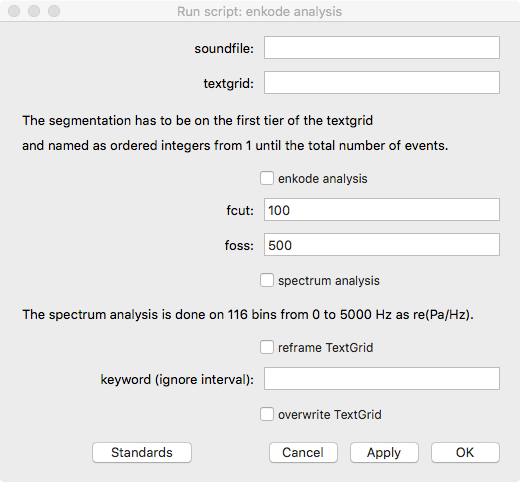
\includegraphics[scale=0.5]{img/5612}
		\caption{The ScriptEditor window of the script \texttt{enkode.praat}.}
		\label{fig:praat}
	\end{center}
\end{figure}

\section{\textit{Addendum}}
\subsection*{Roughness}

An additional option aims to estimate some kind of roughness. Note that is comprehensively empirical and does not take into account the psycho-acoustic phenomenon, but allows certain relevance in certain situation for sound discrimination for instance. This consists to estimate an emergent frequency from the peaks of the loudness analysis. An accurate time step is required and set at 0.001s by default, that is to say a factor of 0.1 of the analysis time step of \textsl{enkode}. The result is a raw data and have to be interpreted knowing that the roughness is identified as such and as a subjective perception in the range of 15 Hz (below this value, we are talking about vibrato) to 300 Hz (beyond that the effect disappears) with a maximum at 70 Hz\footnote{This can be interpreted as follow :\\ \indent \quad $roughness = e^{-0.00355 (midinote-37.175)^2}$\\ \indent \quad with $midinote=12 \cdot log_2(frequency \times 0.00227272727) + 69$.\\ \indent See appendice \fullref{rugdoc} to know more about roughness in psychoacoustic.}. Each value is evaluated as the average of the first derivative of the peaks curve, and correlated with a reliability as the mean value of the standard deviation of the first derivative, which is normalised in order to subtract this value to one as a percentage of confidence.
